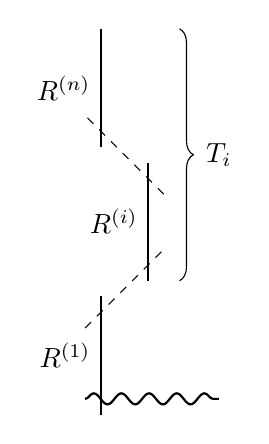
\begin{tikzpicture}
  \draw[thick,decorate,decoration={snake,amplitude=2pt}] (-.2,.2) -- (1.5,.2);
  \draw[thick] (0,0) -- node[left]{$R^{(1)}$} (0,1.5);
  \draw[dashed] (-.2,1.1) -- (.8,2.1);
  \draw[thick] (.6,1.7) -- node[left]{$R^{(i)}$} (.6,3.2);
  \draw[dashed] (.8,2.8) -- (-.2,3.8);
  \draw[thick] (0,3.4) -- node[left]{$R^{(n)}$} (0,4.9);
  \draw [decorate,decoration={brace,amplitude=5pt,mirror}] (1,1.7) -- (1,4.9) node [midway,xshift=.5cm]{$T_i$};
 \end{tikzpicture}